\section{Results}

% Questions to answer:
% How well is your model performing vs. baseline?
% What other ways might you measure its success/failure?
% Why is your model making the errors it is? 
% Back up your claims with empirical evidence
% At least one table with datasets as rows and experiments as columns

% TODO Add a subsection discussing the results of the SAE fine tuning. What was the MSE loss and accuracy. Maybe add 1-2 visuals.

% TODO Consider adding some brief stats about the SAEs reconstruction performance. Basically, how well does it reconstruct/emulate activations from the original transformer?

% The following table was moved to the appendix and expressed as bullet point sentences:
% \begin{table}[h]
% \centering
% \begin{tabular}{|l|r|}
% \hline
% \textbf{Metric} & \textbf{Value} \\
% \hline
% Number of training tokens & 61,440,000 \\
% Overall loss & 211.71364 \\
% MSE loss & 66.29448 \\
% L1 loss & 29.08383 \\
% CE loss score & 0.99386 \\
% Explained variance & 0.89557 \\
% L2 ratio (out/in) & 0.79866 \\
% Mean log10 feature sparsity & -3.22845 \\
% Dead features & 66 \\
% \hline
% \end{tabular}
% \caption{Key Metrics from Custom SAE Training}
% \label{tab:autoencoder_metrics}
% \end{table}

% Our experiment involved extracting features from two sparse autoencoders and evaluating them using a combination of keyword matching, human evaluation, coherence scoring, and an intervention test using vector steering. We determine a feature to be of interest if at least two of the top token-activating tokens occur in our reference vocabulary. The reference vocabulary contains common medical terms put together using a combination of an LLM and the Wiki Medical Terms dataset\hyperlink{med-gpt2}{[4]}.

% The resultant feature set for each model is then evaluated for sharpness. Intuitively, a feature is sharp if the top activating tokens are highly correlated, giving the feature a clear sense of purpose or identity. We empirically ground this intuition using a novel metric we call "semantic coherence." The semantic coherence score provides a comprehensive measure of the semantic relatedness of a neuron's top-K activations. Unlike cosine similarity, which compares two vectors directly, this score considers all pairwise comparisons between the embeddings of the top-K activated tokens. It weights these comparisons by the product of the tokens' activation scores, giving more importance to strongly activated pairs. The score is normalized by the total weight to produce a value between 0 and 1, where higher values indicate greater semantic coherence. This method captures the overall semantic consistency of a neuron's behavior across multiple activations, in contrast to cosine similarity, which only measures the similarity between two specific vectors. By incorporating activation strengths and aggregating multiple pairwise comparisons, the semantic coherence score provides a more nuanced and context-aware evaluation of a neuron's semantic properties than simple cosine similarity.



%%%%%%%%%%%%%%%%%%%%%%%%%%%%%%%%%%%%%%%%
% Our experiment involved extracting features from two sparse autoencoders and evaluating them using keyword matching, human evaluation, coherence scoring, and a vector steering intervention test. A feature is of interest if at least two of the top activating tokens occur in our reference vocabulary, which contains common medical terms compiled using an LLM and the Wiki Medical Terms dataset \hyperlink{med-gpt2}{[4]}.

% Each model's feature set is then evaluated for sharpness. A feature is considered sharp if its top activating tokens are highly correlated, indicating a clear purpose or identity. We measure this using a novel"semantic coherence" score, which evaluates the semantic relatedness of a neuron's top-K activations. This score, ranging from 0 to 1, considers all pairwise comparisons between the embeddings of the top-K activated tokens, weighted by the product of their activation scores. It captures the overall semantic consistency of a neuron's behavior across multiple activations, providing a more nuanced evaluation than simple cosine similarity.

% Mathematically, we define the semantic coherence score as follows:

% \begin{equation}
% \text{Coherence Score} = \frac{\sum_{i=1}^{n-1} \sum_{j=i+1}^n w_i w_j \cdot \text{sim}(\vec{e_i}, \vec{e_j})}{\sum_{i=1}^{n-1} \sum_{j=i+1}^n w_i w_j + \epsilon}
% \end{equation}

% Where:
% \begin{itemize}
%     \item $n$ is the number of valid tokens in the top-K activated tokens
%     \item $w_i$ and $w_j$ are the activation scores for tokens $i$ and $j$ respectively
%     \item $\vec{e_i}$ and $\vec{e_j}$ are the word embeddings for tokens $i$ and $j$ respectively
%     \item $\text{sim}(\vec{e_i}, \vec{e_j})$ is the cosine similarity between embeddings $\vec{e_i}$ and $\vec{e_j}$, calculated as:
%     \begin{equation}
%     \text{sim}(\vec{e_i}, \vec{e_j}) = 1 - \text{cosine\_distance}(\vec{e_i}, \vec{e_j})
%     \end{equation}
%     \item $\epsilon$ is a small constant (e.g., $10^{-8}$) to avoid division by zero
% \end{itemize}

% The cosine similarity is defined as:
% \begin{equation}
% \text{sim}(\vec{e_i}, \vec{e_j}) = 1 - \frac{\vec{e_i} \cdot \vec{e_j}}{\|\vec{e_i}\| \|\vec{e_j}\|}
% \end{equation}
%%%%%%%%%%%%%%%%%%%%%%%%%%%%%%%%%%%%%%%%

Our experiment evaluated features from two sparse autoencoders using keyword matching, human evaluation, coherence scoring, and vector steering intervention. Features of interest are those with at least two top activating tokens present in our reference medical vocabulary \hyperlink{med-gpt2}{[4]}.

We assess feature sharpness using a novel "semantic coherence" score, which measures the semantic relatedness of a neuron's top-K activations. This score (0-1) evaluates pairwise comparisons between embeddings of top-K activated tokens, weighted by their activation scores, capturing the neuron's semantic consistency across multiple activations.

The semantic coherence score is defined as:

\begin{equation}
\text{Coherence Score} = \frac{\sum_{i=1}^{n-1} \sum_{j=i+1}^n w_i w_j \cdot \text{sim}(\vec{e_i}, \vec{e_j})}{\sum_{i=1}^{n-1} \sum_{j=i+1}^n w_i w_j + \epsilon}
\end{equation}

Where $n$ is the number of valid tokens, $w_i$ and $w_j$ are activation scores, $\vec{e_i}$ and $\vec{e_j}$ are word embeddings, and $\text{sim}(\vec{e_i}, \vec{e_j})$ is the cosine similarity between embeddings. $\epsilon$ is a small constant to avoid division by zero.


\subsection{Intervention Test Results}

For the intervention experiment, we evaluate one feature at a time by attaching a steering vector that amplifies the corresponding neuron weights and generating sequences (up to 50 tokens). We then assess the output's cosine similarity to the feature's top-K tokens. Amplifying sparse feature weights should increase the representation of these tokens proportional to the steering vector coefficient. We interpret the steered output by comparing it to the model's normal (un-steered) output.

In our baseline model, we extracted 24,576 features from the eighth attention block's residual stream and identified 101 features of interest. These were filtered through keyword matching against a reference vocabulary and human evaluation. Of these, 100 (99\%) produced steered output with higher semantic similarity than the un-steered counterpart, indicating high receptivity to vector steering using a coefficient multiplier of 50 based on basic parameter optimization techniques. For the fine-tuned model, we extracted the same number of features and identified 111 relevant features. Of these, 93 (83.7\%) produced steered output with higher similarity scores than the un-steered output.

% In our baseline model, we extracted 24,576 features from the residual stream of the eighth attention block. Of these, we identified 101 features related to the subject of interest. These were filtered based on keyword matching against a reference vocabulary containing tokens of interest and further evaluated by a human. Of the 101 features matched through a combination of keyword matching and human evaluation, 100 (99\%) produced steered output that achieved a higher semantic similarity than the un-steered counterpart, suggesting that overall 99\% of the identified features of interest were receptive to vector steering. We used a coefficient multiplier of 50. % TODO: Add a section about how we scaled the coefficient for the fine-tuned model based on the mean increase in activation value

% We extracted the same number of features (24,576) from the same hook point of the fine-tuned model. 111 features were identified using the same process previously described (i.e., keyword matching and human evaluation). 93 (83.7\%) produced steered output that achieved a higher similarity score than the un-steered output.

% \begin{table}[h]
% \centering
% \begin{tabular}{lcccc}
% \hline
% \multirow{Vector Steering Results} & \multicolumn{2}{c}{Model 1 (Baseline)} & \multicolumn{2}{c}{Model 2 (Fine-tuned)} \\
% \cline{2-5}
%  & Value & Percentage & Value & Percentage \\
% \hline
% Total medical domain features & 101 & 0.39\% & 111 & 0.43\% \\
% Features passing intervention test & 100 & 99\% & 93 & 84\% \\
% Average steered similarity & 0.6118 & - & 0.5165 & - \\
% Average baseline similarity & 0.4634 & - & 0.4651 & - \\
% \hline
% \end{tabular}
% \caption{Summary of intervention results for baseline and fine-tuned models}
% \label{tab:intervention_results}
% \end{table}

% \begin{table}[h]
% \centering
% \small
% \begin{tabular}{lcc}
% \hline
% \textbf{Model 1 (Baseline)} & Value & Percentage \\
% \hline
% Total medical domain features & 101 & 0.39\% \\
% Features passing intervention test & 100 & 99\% \\
% Average steered similarity & 0.6118 & - \\
% Average baseline similarity & 0.4634 & - \\
% \hline
% \end{tabular}
% \caption{Vector Steering Results - Baseline Model}
% \label{tab:intervention_results_baseline}
% \end{table}

% \begin{table}[h]
% \centering
% \small
% \begin{tabular}{lcc}
% \hline
% \textbf{Model 2 (Fine-tuned)} & Value & Percentage \\
% \hline
% Total medical domain features & 111 & 0.43\% \\
% Features passing intervention test & 93 & 84\% \\
% Average steered similarity & 0.5165 & - \\
% Average baseline similarity & 0.4651 & - \\
% \hline
% \end{tabular}
% \caption{Vector Steering Results - Fine-tuned Model}
% \label{tab:intervention_results_finetuned}
% \end{table}

\begin{table}[h]
\centering
\footnotesize
\begin{tabularx}{\columnwidth}{@{}lXX@{}}
\toprule
\textbf{Metric} & \textbf{Baseline} & \textbf{Fine-tuned} \\
\midrule
Total medical features & 101 (0.39\%) & 111 (0.43\%) \\
Passing intervention & 100 (99\%) & 93 (84\%) \\
Avg. steered similarity & 0.6118 & 0.5165 \\
Avg. baseline similarity & 0.4634 & 0.4651 \\
\bottomrule
\end{tabularx}
\caption{Vector Steering Results Comparison}
\label{tab:intervention_results}
\end{table}

\subsection{Coherence Scores}

We contrast the features of the baseline model with those of the fine-tuned model by comparing their coherence scores. When comparing the entire feature set, we observe that the mean coherence scores of the baseline features (0.5438) are higher than those of the fine-tuned features (0.3511), with a difference of 0.1927.

To contextualize this difference, we normalized it with respect to the range of coherence scores. The baseline model's coherence scores range from 0.1130 to 0.7641, while the fine-tuned model's scores range from 0.0615 to 0.6793. The normalized mean difference is 0.3037, indicating that the difference in coherence scores is approximately 30.37% of the average range of scores across both models.

% \begin{table}[h]
% \centering
% \begin{tabular}{lcc}
% \hline
% \textbf{Metric} & \textbf{Mean} & \textbf{Median} \\
% \hline
% Coherence Score (Model 1 - Baseline) & 0.5438 & 0.5648 \\
% Coherence Score (Model 2 - Finetuned) & 0.3511 & 0.3196 \\
% Difference (Baseline - Finetuned) & 0.1927 & 0.2452 \\
% \hline
% \end{tabular}
% \caption{Comparison of Coherence Scores between Baseline and Finetuned Models}
% \label{tab:coherence_scores}
% \end{table}

\begin{table}[h]
\centering
\footnotesize
\begin{tabularx}{\columnwidth}{@{}lXX@{}}
\toprule
\textbf{Metric} & \textbf{Mean} & \textbf{Median} \\
\midrule
Baseline Coherence & 0.5438 & 0.5648 \\
Finetuned Coherence & 0.3511 & 0.3196 \\
Difference & 0.1927 & 0.2452 \\
\bottomrule
\end{tabularx}
\caption{Coherence Scores Comparison}
\label{tab:coherence_scores}
\end{table}

The substantial difference in coherence scores suggests that fine-tuning has significantly altered the feature representations in the model. Lower coherence scores in the fine-tuned model might indicate that features have become more specialized or task-specific, potentially at the cost of general coherence. Further investigation into these changes and their impact on model performance is needed to understand the effects of fine-tuning on feature representations.

Figure 1 shows the distribution of medically-related terms among each feature's top-K activating tokens. Medically-related features are defined as those with at least 2 of their top 10 activating tokens matching our reference medical vocabulary. While the fine-tuned model has more medically-related features, the baseline model shows a broader distribution with higher numbers of medical term matches. Notably, the baseline model has features with 7 or more medical tokens in their top-K set, which is absent in the fine-tuned model. This aligns with the finding of lower mean coherence scores for medical features in the fine-tuned model, as coherence scores are influenced by the number of medical tokens in a feature's top activating set. This explains the observed distribution pattern and provides insight into the differing representations of medical knowledge between the models.
\begin{figure}[htbp]
    \centering
    \vspace{-1em} % Reduces space above the figure
    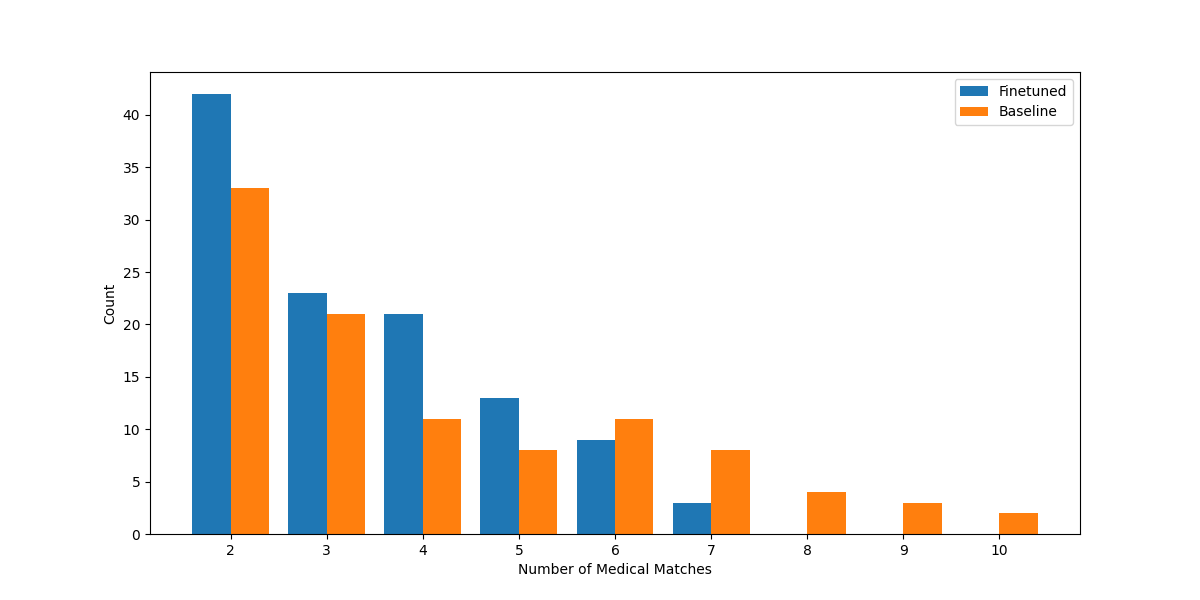
\includegraphics[width=0.8\linewidth]{dist-of-keyword-matches.png}
    \vspace{-1em} % Reduces space below the figure
    \caption{Distribution of medical term matches in top-K activating tokens for features in fine-tuned and baseline models}
\end{figure}


% The paragraph below is redundant:
% Uniform efficacy of the causal intervention is not guaranteed for the two feature sets. We suspect that models are more responsive to steering vectors when the top activating tokens for the respective feature are more semantically similar to one another. The semantic coherence score reflects this by accounting for n-gram semantic similarities as well as the activation values. We find this approach to be more robust than basic cosine similarity scoring as it also accounts for the weighted token activation values. 

% TODO remove if we can't do regression:
% To gauge the effect of coherence scores on the model's proclivity towards vector steering responsiveness, we regress feature coherence scores on vector steering outcomes.
% [TODO: Add stargazer table and brief discussion of the regression results]

\subsection{Word Analysis} % Probably should rename this to something better

Our analysis revealed significant differences in the features extracted by the sparse autoencoder (SAE) from the baseline and fine-tuned models. 1.1 times as many medically-related features were extracted from the fine-tuned model compared to the baseline model. Specifically, we identified 111 medical features in the fine-tuned model versus 101 in the baseline model.

The mean activation values for medically related features differed substantially between the two models. In the fine-tuned model, we observed a mean activation of $\mu$ = 0.794 with a variance of $\sigma^{2}$ = 0.018, while the baseline model showed a mean activation of $\mu$ = 2.166 with a variance of $\sigma^{2}$ = 0.633. These statistics indicate that the fine-tuned model's medical features have lower mean activation values and significantly reduced variance compared to the baseline model.

The activation distributions revealed notable differences: the fine-tuned model's activation values form a sharp, narrow normal curve, indicating more consistent activation of medical features. In contrast, the baseline model shows a broader normal distribution with more varied activation patterns. Comparative analysis highlights these differences: the fine-tuned model has 97.16\% lower variance and 63.34\% lower mean activation strength compared to the baseline model. These results suggest that fine-tuning has created a more specialized representation of medical knowledge, with consistently activated features, unlike the baseline model, which has fewer but more variable medical features.

\begin{figure}[htbp]
    \vspace{-1em} % Reduces space above the figure
    \centering
    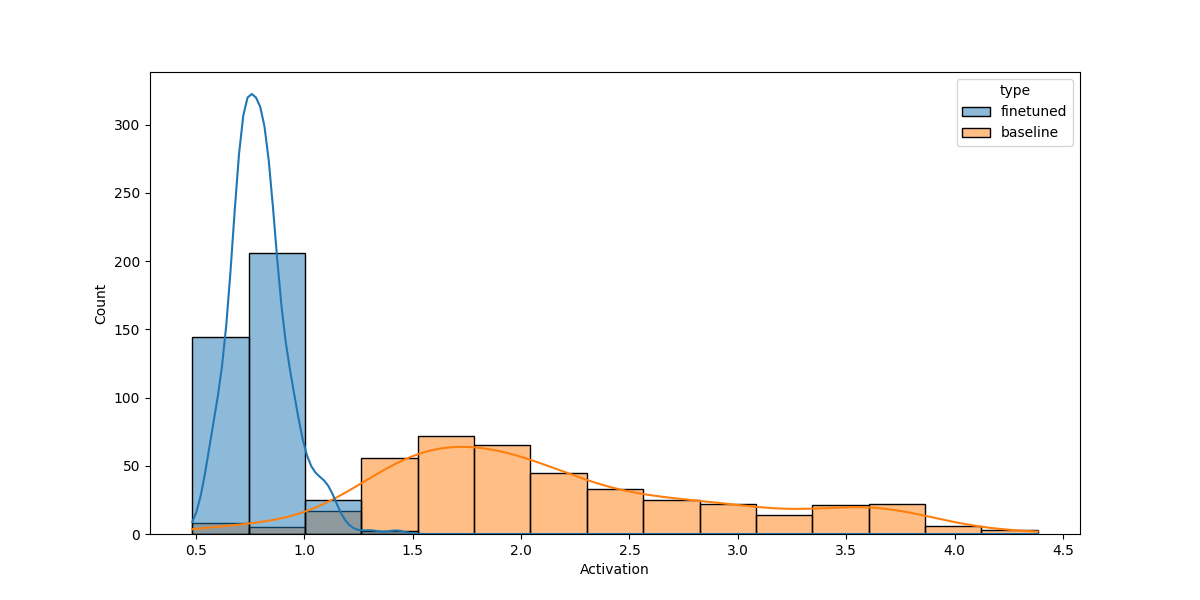
\includegraphics[width=0.9\linewidth]{dist_acts_for_medical_words-no-title.png}
    \vspace{-1em} % Reduces space below the figure
    \caption{Distribution of Activation Values for Medical Words}
\end{figure}


%%%%%%%%%%%%%%%%%%%%%%%%%%%%%%%%%%%%%%%%%%%%%%%%%%%%%%%%%%%%%%%%%%%%%%%%
\subsection{Discussion}
%%%%%%%%%%%%%%%%%%%%%%%%%%%%%%%%%%%%%%%%%%%%%%%%%%%%%%%%%%%%%%%%%%%%%%%%

We also tested our approach on a custom fine-tuned GPT2 model, though we don't include those results here.\hyperlink{old-finetuned-results}{[5]} Like the other fine-tuned model, this model under-performed the baseline on the intervention test. We hypothesize that fine-tuning may make models less responsive to vector steering interventions. This could be because fine-tuning skews the data distribution, reducing the balance typically observed in pre-trained foundation models. The elevated mean activation score observed in the fine-tuned model supports this theory. It is possible that a fine-tuned model trained with more rigor may yield lower, more normally distributed activation scores. Regression analysis may be effective approach to further contextualizing the effect of activation score distributions on vector steering efficacy.

Notably, our coherence scoring algorithm is limited by the word embedding model selection. Each coherence score calculation involves computing the cosine similarity of the word embedding for each feature's top-K activating tokens. Our models were trained using a sub-word tokenizer, resulting in a fairly substantial vocabulary gap. Specifically, the features of interest (i.e., the features related to medical terms) extracted from the baseline model achieved a word embedding coverage of 84.51\% (unique) and 89.99\% Coverage (total). Unique coverage refers to the number of distinct words in the feature set, without considering how many times each word appears. Total coverage is total count of all words, including repetitions. Two contending word embedding models, "fasttext-wiki-news-subwords-300" and "word2vec-google-news-300", were evaluated as well. In both cases, the "glove-wiki-gigaword-100" model performs the best, despite having fewer dimensions (100) compared to the other models (300). A potential area for future research could be exploring ways to close this coverage gap by using word embeddings trained specifically on the SAE's feature activation corpus.